\documentclass[a4paper,10pt,twoside]{article}
\title
{
\LARGE BITS F464 Machine Learning \\
\LARGE Fischer's Linear Discriminant
}
\usepackage[left=2cm, right=2cm, top=1.5cm]{geometry}
\usepackage{xcolor}
\usepackage{ragged2e}
\usepackage{comment}
\usepackage{graphicx}
\usepackage{subfig}
\usepackage{amsmath, amsfonts}
\usepackage[english]{babel}
\date{}
\author{}
\begin{document}
\maketitle
%===================================================================================================================%
\section*{\textcolor{blue}{1. Introduction:}}
In this report, we try to analyse the performance (accuracy and fscore) of a Fischer's Linear Discriminant. The implementation of this model was done using Jupyter Notebook, NumPy, Pandas and Matplotlib.

\section*{\textcolor{blue}{2. Procedure:}}
\begin{enumerate}
\item{The given dataset was initially split into two classes, positive and negative, according the target variable.}
\item{The mean and covariance matrix for both classes was found and the overall covariance matrix $S_W$ was obtained as the sum of covariance matrices of the positive and negative classes, i.e. $S_W$ = $S_1$ + $S_2$.}
\item{The hyperplane onto which the points had to be collapsed was found using the equation W = $S_W^{-1}(m_2 - m_1)$, where $m_2$ and $m_1$ represented the means of the positive and negative classes.}
\item{Next, the points were reduced to 1D by taking a dot product of the direction ratios of the vectors (points in nD) and the direction ratios of the hyperplane ($W$). The points after being reduced to 1D were plotted with positive points having red color and negative having blue color (as shown below).}
\item{The guassian curves were plotted for both classes (with the reduced 1D feature as input) and the point of intersection was found by solving the resulting quadratic (say $\alpha$).}
\item{Now, the point $\alpha$ is the discriminating point in the reduced 1D space. The discrimating line passing through that point has been shown below. The differentiating hyperplane equation is found in the original feature space using $W^T\alpha$. A point was classified as negative if it was to the left of $\alpha$ and positive if it was to the right of $\alpha$}
\item{Finally, the confusion matrix for the model was generated accuracy and fscore values were calculated. The model achieved $99.3\%$ accuracy on dataset-1 and $100\%$ accuracy on dataset-2 (results shown below).}
\end{enumerate}

\newpage
\section*{\textcolor{blue}{3. Results:}}
\begin{figure}[h!]
\centering
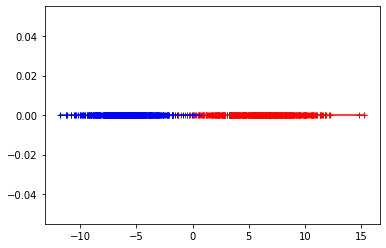
\includegraphics[scale=1.0, width=5cm]{Fig1.png}
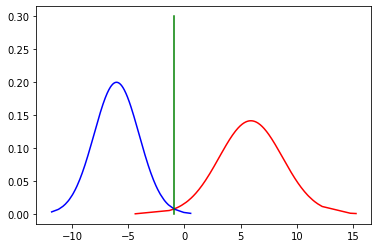
\includegraphics[scale=1.0, width=5cm]{Fig2.png}
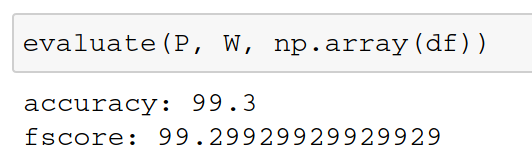
\includegraphics[scale=1.0, width=5cm]{Fig11.png}
\caption{Dataset-I}
\end{figure}

\begin{figure}[h!]
\centering
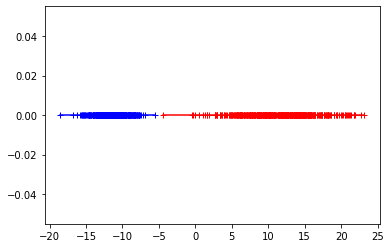
\includegraphics[scale=1.0, width=5cm]{Fig3.png}
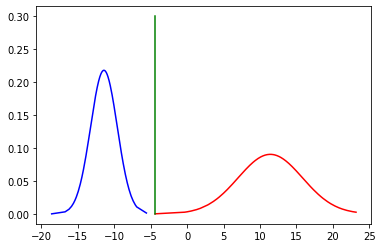
\includegraphics[scale=1.0, width=5cm]{Fig4.png}
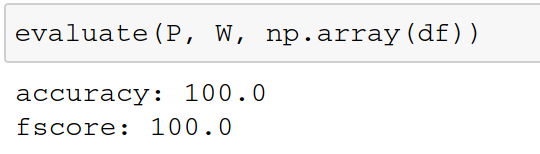
\includegraphics[scale=1.0, width=5cm]{Fig21.png}
\caption{Dataset-II}
\end{figure}
%=================================================================================================================%
\end{document}
